
% This is LLNCS.DEM the demonstration file of
% the LaTeX macro package from Springer-Verlag
% for Lecture Notes in Computer Science,
% version 2.4 for LaTeX2e as of 16. April 2010
%
\documentclass{llncs}
%
\usepackage{makeidx}  % allows for indexgeneration
\usepackage{graphicx}
\usepackage[utf8]{inputenc}
\usepackage{moreverb}
\usepackage{listings}
\usepackage{graphicx}
\usepackage{caption}
\usepackage{subcaption}
\captionsetup{compatibility=false}
\usepackage{algorithm}
\usepackage{algorithmic}
\newcommand{\todo}[1]{\textbf{ToDo: \textit{#1}}}
%\newcommand{\comm}[1]{\textbf{Comment: \textit{#1}}}\stackrel{\leftrightarrow}{}
\usepackage{natbib}
\usepackage{enumitem}
\usepackage[usenames,dvipsnames]{color}
\newcommand{\sparqlwo}[2]{{\texttt{#1 \char '173} \\[1.5pt] \hspace*{.5cm}\parbox{6cm}{\tt #2} \\ \texttt{\char '175} }}
\newcommand{\sparql}[3]{{\texttt{#1 \char '173} \\[1.5pt] \hspace*{.5cm}\parbox{6cm}{\tt #2} \\ \texttt{\char '175} \\ \texttt{#3} }}
\newcommand{\slot}[3]{$\langle\texttt{#1},\text{#2},\text{\sf #3}\rangle$}
\newcommand{\argmax}{\operatornamewithlimits{arg\,max}}
\newcommand{\argmin}{\operatornamewithlimits{arg\,min}}
\usepackage{amssymb}
\usepackage{qtree}
\usepackage[usenames,dvipsnames,table]{xcolor}
\newcommand{\Drs}[2]{%%%%%%%%%%%%%%%%%%%%%%%%%
\(                   % begin maths mode
 \begin{array}{|l|}  %
 \hline              % top line
   \begin{array}{l}  %
    #1                % `Universe'
    \end{array} \\   %  end the `universe' part
 \hline              % line between Universe and Conditions
    \begin{array}{l} %
    #2                % the conditions
    \end{array} \\   % end the conditions part
 \hline              % bottom line
\end{array}          %
\)                   % end maths mode
                     }%%%%%%%%%%%%%%%%%%%%%%%%%
%
\begin{document}
%
\frontmatter          % for the preliminaries
%
\pagestyle{headings}  % switches on printing of running heads
\addtocmark{DAW2} % additional mark in the TOC
%

\vspace{1cm}

\mainmatter              % start of the contributions
%

\title{DAW2: Duplicate-AWare Federated Query Processing over the Web of DAta}
%
\titlerunning{DAW2}  % abbreviated title (for running head)
%                                     also used for the TOC unless
%                                     \toctitle is used
%
\author{Muhammad Saleem\inst{1} \and Axel-Cyrille Ngonga Ngomo\inst{2}
\and Josiane Xavier Parreira\inst{1} \and Manfred Hauswirth\inst{1}}
%
\authorrunning{saleem et al.} % abbreviated author list (for running head)
%
%%%% list of authors for the TOC (use if author list has to be modified)
%\tocauthor{Ivar Ekeland, Roger Temam, Jeffrey Dean, David Grove,
%Craig Chambers, Kim B. Bruce, and Elisa Bertino}
%
\institute{Digital Enterprise Research Institute, National University of Ireland, Galway\\
\email{\{muhammad.saleem, josiane.parreira, manfred.hauswirth\}@deri.org}
\and
Universit\"at Leipzig, IFI/AKSW, PO 100920, D-04009 Leipzig \\
\email{ngonga@informatik.uni-leipzig.de}
}

\maketitle              % typeset the title of the contribution

\begin{abstract}
Over the last years, the Web of Data has developed into a large compendium of interlinked data sets from multiple domains.
Due to the decentralised architecture of this compendium, several of these data sets contain duplicated data.
A number of federated querying approaches have been proposed to retrieve information from the Data Web.
Still, only little attention has been paid to the effect of duplicated data on the processing of federated queries.
This work presents DAW2, a novel duplicate-aware approach to federated SPARQL querying based on Min-Wise Independent Permutations (MIPs) applied to RDF predicates.
%Our approach begins by parsing each input query for triple patterns.
%Then, for each of these triple patterns, it uses MIPs to approximate the amount of non-duplicate triples contained in each of the available data sources. 
%This approximation is used to select and rank relevant data sources. 
%Finally, the selected data sources are queried by means of the sub-queries contained in the user input.
DAW2 allows taking into account the overlap among the available data sources and thus avoid submitting sub-queries that produce overlapping results.  
Our approach can be combined with existing federated query engines and enables them to achieve the same recall while submitting fewer queries. 
Consequently, DAW2 can reduce both the overall runtime of and the amount of network traffic generated by federated query engines.
%DAW2 can be combine with the existing federated approaches can achieve similar performance while using fewer sub-queries, thus improving both execution time and network traffic. 
%Moreover, our approach queries the data sources by using single triple patterns and can thus also retrieve results whose fragments are distributed across the Web of Data.
%We develop a duplicate-aware federated query engine by extending DARQ (a well-known federated engine) and evaluate by using four datasets of different sizes and a total of 79 queries of various shapes. 
We extend both DARQ and SPLENDID with our DAW2 and compare our extensions with the original implementation of these frameworks on four datasets of different sizes by using 79 queries of various shapes. 
Our evaluation shows that our extensions achieve significantly smaller mean squared errors than the original implementations with respect to the approximation of result set sizes as well as in the ranking of data sources. 
%Our evaluation shows that our approach achieves significantly smaller mean squared errors with respect to the approximation of result set sizes as well as in the ranking of data sources. 
Moreover, our extensions require less sub-queries as well as a smaller execution time to achieve the same recall.
\keywords{Federated queries, SPARQL, Min-wise independent permutations}
\end{abstract}
%
\section{Introduction}
Over the last years, the Data Web has developed into a large compendium of interlinked data sets from multiple domains~\cite{AUE+11}. 
One of the central principles underlying the architecture of these data sets is the reuse of URIs and vocabularies as well as the linking of knowledge bases~\cite{key-20}.
One of the results of this architectural choice is that certain queries can only be answered by retrieving information from several knowledge bases.
This type of queries, called \emph{federated queries}, is of central importance for manifold applications such as question answering~\cite{UNG+12} and knowledge retrieval~\cite{SHE+11}.
Due to the reuse of URIs and the independence of the data sources, certain pieces of information (i.e., triples) can be found in several knowledge bases. 
For example, the name of movie directors can be found both in DBpedia and LinkedMDB.
Authors of papers can be found in both the ACM and DBLP libraries. 
Similarly, we have noticed that the \emph{DrugBank}\footnote{\url{http://datahub.io/dataset/fu-berlin-drugbank}}
and \emph{Neurocommons}
\footnote{\url{http://neurocommons.org/page/RDF\_distribution}} 
datasets are duplicated at \emph{DERI health Care and Life Sciences Knowledge Base}
\footnote{\url{http://hcls.deri.org:8080/openrdf-sesame/repositories/hclskb}}. 
A list of the mirrored SPARQL endpoints is given in the url
\footnote{\url{http://hcls.deri.org/RoadMapEvaluation/\#Sparql\_Endpoints}}. 
These duplicates are common in life sciences domain as well.  
Examples of data sets which might contain the same triples across the life science domain is shown in Figure~\ref{fig:datasets}. 
We call triples that can be found in several knowledge bases across the Web of Data \emph{duplicates}. 

%It is important to make a distinguish between fragmented and duplicated data. 
%We speak of \emph{fragmented data}, when different set of information about the same resource is stored in different datasets. 
%For example, while the side-effects of drugs can be found in Sider\footnote{\url{http://datahub.io/dataset/fu-berlin-sider}}, the specifics of a drug (such as its INCHI key) can be found in Drugbank while the data on the companies that produce the drugs are in Dailymed\footnote{\url{http://datahub.io/dataset/fu-berlin-dailymed}}. 
%While duplicate data mean, the same set of information about a resource is stored in multiple data sets available via different SPARQL endpoints.

Avoiding the retrieval of duplicate records is a crucial issue in large scale distributed datasets. As the SPARQL endpoints are autonomous, there is always the possibility of high mutual overlap between different datasets residing in different endpoints. It is thus likely that an optimized query execution plan contains a sub-query that retrieves records which are already retrieved by another sub-query from a different SPARQL endpoint. In this case it is not necessary to execute the later sub-query, as it would not only result in duplicate records being retrieved but also increase the total processing time.

While the importance of federated queries over the Web of Data has been stressed in previous work, the impact of duplicates has not received much attention. Yet, as we will show in the remainder of this paper, a duplicate-aware approach to query processing can lead to more time-efficient and effective algorithms for federated queries.
In this paper, we address this drawback by presenting a duplicate-aware approach for query processing based on Min-Wise Independent Permutations (MIPs). Our query federator makes
use of MIPs to estimate the possible
overlap between the results of different sub-queries in order to avoid the retrieval of redundant information.

Our approach begins by parsing each input query for triple patterns.
Then, for each of these triple patterns, it uses MIPs to approximate the amount of non-duplicate triples contained in each of the available data sources. 
This approximation is used to select and rank relevant data sources. 
Finally, the selected data sources are queried by means of the sub-queries contained in the user input.


The use of statistical synopsis such as MIPs for overlap estimation is very common in the literature (as discussed in the next section), however these synopsis cannot be use all alone in semantic web domain due to the diverse nature of SPARQL queries. For example, the synopsis result set estimation for a triple pattern needs to be completely changed if any of the subject or object becomes bound in the query triple. To address such issues, we combine MIPs synopsis with the data summaries statistics for more accurate overlap estimation. Thus by creating small summaries of the data found in the available knowledge bases, our approach is able to estimate the amount of new information contained in a knowledge base with a high accuracy, leading to a better performance with respect to source ranking, estimation of result set sizes, execution time and network traffic. 

The main contributions of this paper are as follows:
\begin{enumerate}
\item We propose the (to the best of our knowledge) first duplicate-aware approach for federated SPARQL querying.
\item We combine data summaries statistics with MIPs to address the diversity in SPARQL queries.
\item We evaluate our approach against the state of the art on 79 queries and four datasets and show that we achieve better estimations of result set sizes and therewith a better ranking of data sources, lower execution times and consequently less network traffic.
\end{enumerate}
%
%An experimental evaluation on 79 queries shows that our approach outperforms the state-of-the-art by retrieving the same data with less queries. 
The rest of this paper is organized as follows: 
We begin by giving a brief overview of the state of the art in federated query processing.
In addition, we present different statistical synopsis approaches that can be used for the approximation of duplicate-free result set sizes. 
Thereafter, we elaborate on our novel duplicate-aware federated query processing approach and present the components of our approach in detail.
Subsequently, we present a thorough evaluation of our approach against state of the art approaches.
We finally conclude the paper with a discussion of our findings and an overview of future work.
\begin{figure}
\centering
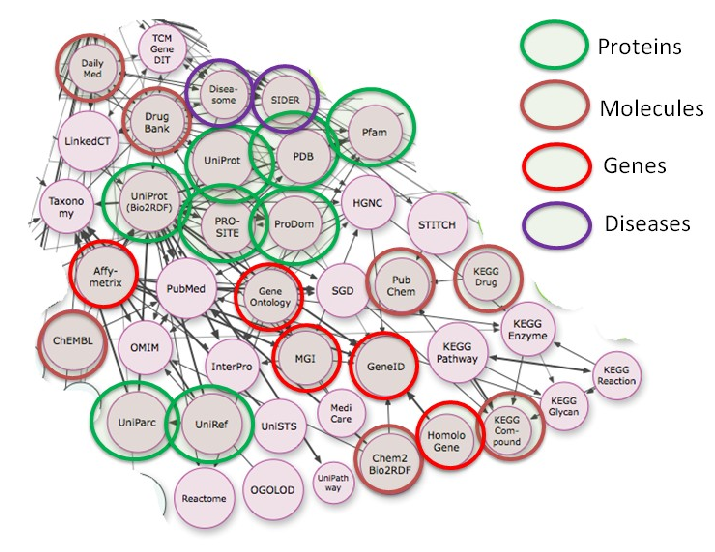
\includegraphics[scale=0.70]{img/possibleDuplicates} 
\caption{Possible duplicates in life sciences domain}
\label{fig:datasets}
\end{figure}

\section{Related Work}
\subsection{Federated SPARQL Queries}
The research work on federated query processing over the Data Web
can be categorized into three main directions: 
\begin{itemize}
\item Service description/index-assisted approaches, which make use of the dataset summaries that have been collected in a pre-processing stage. These approaches may lead to a more efficient query federation. However,
the index needs to be constantly updated to ensure up-to-date results.
Also, the index size should not be large to ensure that it does not
increase the overall query processing cost. 
\item Index-free approaches, in which the query federation is performed
without using any stored data summaries. The data source statistics can be collected on-the-fly before the query federation. This approach promises the up-to-date records retrieval however; it may increase the query execution time, depending on the extra processing required in collecting, processing on-the-fly statistics.
\item Hybrid approaches, in which some of the data source statistics are pre-stored while some are collected on-the-fly. 
\end{itemize}

All of the above approaches can be further divided into two categories
(a) Query federation with complete result retrieval (100\% recall), and (b) Query federation
with partial (sufficient) record retrieval. In our work, we focus
on index-assisted query federation which can be used both for complete and partial record retrieval .

Heiner et al.~\cite{key-1} describe how to extend the Sesame RDF
repository to support distributed SeRQL queries over multiple Sesame
RDF repositories. They use a special index structure to determine
the relevant sources for a query. Quilitz and Leser~\cite{key-2}
use the theoretical knowledge of~\cite{key-1} to develop the first federated
query engine (named DARQ) for remote RDF data sources. DARQ uses service
descriptions for relevant data source selection. A service description
describes the capabilities of a SPARQL endpoint. They use a query rewriting
mechanism based on~\cite{key-8} and a cost-based optimization algorithm
to reduce the query processing time with the minimum bandwidth usage.
DARQ is compatible with any SPARQL endpoint that implements the SPARQL
standard. Their experimental results show that the optimization algorithm
can greatly reduce the query processing time.

Andreas et al.~\cite{key-3} propose a solution similar to DARQ using a
mediator approach. The SPARQL endpoints need to register first
with the mediator using HTTP POST requests with an RDF document attached.
The mediator continuously monitors the SPAQL endpoints for any dataset
changes and updates the service descriptions automatically. Unlike
DARQ, the service descriptions remain up-to-date all time. 

Olaf et al.~\cite{key-4} present a new approach for federated query processing
over the Web of Data. Their approach discovers data that might be
relevant for answering a query during the query execution itself.
The discovery of relevant data is accomplished by traversing RDF links.
They use an iterator-based pipeline and a URI prefetching approach
for efficient query execution. Both DARQ and~\cite{key-3} are not able
to discover relevant data sources by the query itself.

The previous techniques cannot answer all types of queries due to
index or service description limitations. Umbrich et al.~\cite{key-5, key-6}, propose a Qtree-based index structure which summarizes the
content of data source for query execution over the Web of Data. Their approach is able to handle more expressive queries however; because of the complete-query based source ranking, it may skip querying many sources which are capable of answering a sub-set of the query triples. Schwarte
et al.~\cite{key-7} propose an index-free query federation for the Web
of Data. Their approach gives a reasonably fast data retrieval as
compared to all the previous techniques. However, since they do not
keep any statistics, it works only for limited data sources.

Li and Heflin~\cite{key-15} build a tree structure which supports federated query processing over multiple heterogeneous sources. They make use of an OWL reasoner to answer queries
over the selected sources and their corresponding ontologies. Kaoudi et al.~\cite{key-16}
propose a federated query technique on top of distributed hash tables (DHT). 
 The overall goal is to minimize the query execution time and the bandwidth
consumption by reducing the cardinality of intermediate results. The DHT-based optimizer make use of three greedy optimization algorithms for best plan selection.  

Ludwig and Tran~\cite{key-18} propose a mixed
query engine that assumes some incomplete knowledge about the sources to select and discover new sources at run time. A Symmetric Hash Join
is implemented to incrementally produce answers. This approach
is extended to query both remote and local linked data~\cite{key-19}.

Maribel et al.~\cite{key-21} present ANAPSID, an adaptive query engine
that adapts query execution schedulers to SPARQL endpoints data
availability and run-time conditions. ANAPSID provides physical SPARQL
operators that detect when a source becomes blocked or data traffic
is bursty. The operators produce results as
quickly as data arrives from the sources. Amol et al.~\cite{key-17} present a survey of the adaptive query processing
techniques, common issues, and the settings in which each piece of work is most appropriate. 
Avalanche~\cite{key-24} gathers endpoints dataset statistics and bandwidth availability on-the-fly before the query federation. The advantage of this technique is the live query execution over the Web of Data. However, on-the-fly statistics calculation can increase the overall query execution time. Olaf~\cite{key-25} propose a heuristics-based technique to minimize query intermediate
results. 

%Other noteable contributions such as LIMES~\cite{key-26}, SILK~\cite{key-27}, EAGLE~\cite{key-28} provides time-efficient approaches for link discovery using
%various distance measure techniques. The LIMES framework utilize the mathematical
%characteristics of metric spaces to compute similarity estimates between
%instances. It makes use of the triangle inequality to partition the
%metric space into different portions. Each of these portions of the
%space is then represented by an exemplar~\cite{key-33} that allows to compute
%an accurate distance approximation between different instances. SILK
%implements a multi-dimensional blocking approach for link discovery.
%The Levenshtein distance~\cite{key-34} is used for approximate for similarity
%estimation between different instances. EAGLE presents a novel active
%learning approach to learning link specifications based on genetic programming.
%EAGLE generates highly accurate link specifications while reducing the
%annotation burden for the user. 

Few other contributions address the problem of SPARQL query federation~\cite{key-22},~\cite{key-23} but none, to the best of our knowledge has taken into account the possibility of mutual overlap between different RDF datasets before query execution. Similar to DARQ engine, we use service
descriptions for query federation. In addition, we store MIPs vector
statistics for each of the indexed data source. Our query federator makes
use of this special statistic information to estimate the possible
overlap between the results of different sub-queries in order to avoid the retrieval of redundant information.

\subsection{Dataset Overlap Estimation}
Avoiding the retrieval of duplicate records is a crucial issue in large scale distributed datasets. As the SPARQL endpoints are autonomous, there is always the possibility of high mutual overlap between different datasets residing in different endpoints. 
It is thus likely that an optimized query execution plan contains a sub-query that retrieves records which are already retrieved by another sub-query from a different SPARQL endpoint. In this case it is not necessary to execute the later sub-query, as it would not only result in duplicate records being retrieved but also increase the total processing time.

Statistical synopsis like min-wise independent permutations~\cite{key-9}, bloom filters~\cite{key-10}, hash sketches~\cite{key-36}, XSKETCH~\cite{key-37}, fractional XSKETCH~\cite{key-38}, and compressed bloom filters~\cite{key-11} have been extensively used in the literature to provide a compacted representation of data sets. Statistical synopsis allow to estimate a number os set operations such as overlap and union without having to compare the original sets directly. For example, Bender et al.~\cite{key-12} propose a technique for predicting the query-specific mutual overlap datasets in a peer to peer network. MIPs have proved to be the more accurate overlap estimation with small bandwidth consumption\cite{key-9} therefore we have chosen them in our approach.  

\section{Notation}
In this section, we present the core of the notation that will be used throughout this paper.
We denote data sources with $S$ and the total number of data sources with $n$. 
The set of all data sets is dubbed $\mathfrak{S}$.
The set of all possible result sets is denoted $R$ while the set of all possible SPARQL queries is labeled with $Q$. 
A data source ranking function $rank: S \times Q \rightarrow \{1 \ldots n\}$ is a function that assigns a ranking to each data source given a particular query $q \in Q$.
Note that for any source ranking function $rank$, we assume that $\forall S, S' \forall q \in Q : S  \neq S' \Longleftrightarrow rank(S, q) \neq rank (S', q)$.
A result set estimation function $est: S \times Q \rightarrow \mathbb{N}$ aims at approximating the size of the result set that will be returned by a given query.
Note that this function plays a crucial role in the processing of federated queries as it is most commonly used to decide upon the ranking of data sources for a given query.
The aim of a federated query system such as the one described in this work is thus to optimize its estimation function $est$ so as to ensure a ranking of the source close to the optimal ranking. %do we really need this sentence?
\section{Duplicate-aware Federated Query Processing }
\subsection{Overview}
 Given a query, it is first parsed, then sent to federator which makes use of the services descriptions directory/index
to decompose the query into duplicate free multiple sub-queries. Each sub-query is optimized to generate an optimized execution plan. The optimized sub-queries are forwarded to the relevant SPARQL endpoints. The results of each sub-query execution are integrated and the final query result set is generated. This architecture for duplicate-aware federated query processing is shown in Figure 2.
\begin{figure}
\begin{centering}
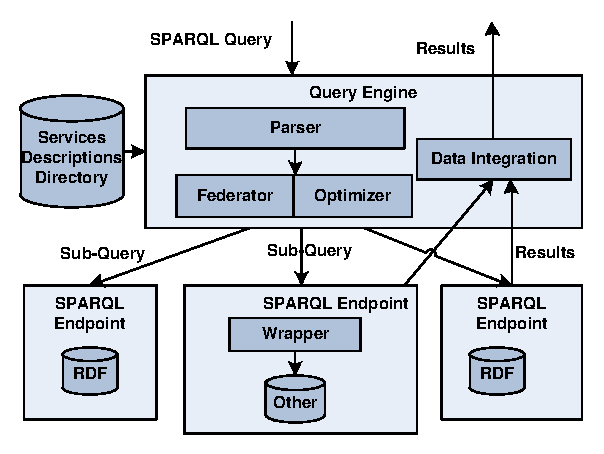
\includegraphics[scale=0.7]{img/Fig1} 
\par\end{centering}
\centering{}\caption{Duplicate-aware federated query processing architecture}
\end{figure}
While this architecture is similar to other federated query systems, the federator in our
system differ significantly from those of other approaches as it
makes use of MIPs statistical information to generate duplicate-free
query execution plans. The generation of MIPs statistical information
is explained in the next section.
\subsection{Service Description Directory}
To find the set of relevant servers and generate 
the appropriate sub-queries, the federator needs information about the
different data sets available at the different servers. We call the catalog containing such information 
the \emph{service description directory}. Each service description
provides a declarative description of the data available from a server
along with statistical information. 

For each server our \emph{service description directory} stores \textit{server url, graph name}, and for
each distinct predicate \emph{p} we record \textit{predicate name,
MIPs vector, subject selectivity, object selectivity}, and \textit{total number of triples} having predicate
\emph{p}. The MIPs vectors are used to estimate the dataset overlap
among the capable datasets before the sub-query distribution and it will be explained in detail in section 4.3. The \emph{subject} and \emph{object selectivity} are used to estimate the sub-query result set when \emph{subject, object} are bound, respectively. We call the set \emph{$C_i = \{(p_i,mipsv_i,sbjsel_i,objsel_i,totTrpl_i)\}$} as a \emph{capability} of the data source. The total number of capabilities of a data source is equal to the number of distinct predicate in that data source. A sample service description is given in the Listing 1.

It is very crucial to keep the directory size small to minimize the pre-query federation time. However,this directory must contain sufficient information to enable the generation of sub-query, the optimization, and the pre-processing dataset overlap estimation. Our index size is mostly depended upon the size of the MIPs vectors which can be adjusted to any length. In general MIPs can provide a good estimation of the overlap between sets with a few integer in length. Min-Wise Independent Permutations have been in the peer to peer networks literature~\cite{key-13, key-39, key-40}.
\begin{lstlisting}[caption = {A Service Description Example},basicstyle={\tiny},float,frame={single},stringstyle={\ttfamily}]
[] a sd:Service ;
     sd:url   <http://localhost:8890/sparql> ;
     sd:graph ``diseasome/DS1'';
     sd:capability
     [
      sd:predicate  diseasome:name ;
      sd:MIPv  ``-6908232 -7090543 -6892373 -7064247 ...'';           
      sd:subjectSelectivity  ``0.0068'' ;
      sd:objectSelectivity  ``0.0069'' ;
      sd:triples    147  ;
      ] ;
     sd:capability
     [
      sd:predicate  diseasome:chromosomalLocation ;
      sd:MIPv  ``-7056448 -7056410 -6845713 -6966021 ...'';
      sd:subjectSelectivity  ``0.0062'' ;
      sd:objectSelectivity  ``0.0072'' ;
      sd:triples    160  ;
      ] ;
\end{lstlisting}
\subsection{Min-Wise Independent Permutations}
MIPs assumes that the set elements can
be ordered and computes N random
permutations of the elements. Each permutation uses a linear hash
function of the form  \emph{$h_i$(x) : = $a_i$*x + $b_i$ mod U} 
where \emph{U} is a big prime number and $a_i$,
$b_i$ are fixed random numbers~\cite{key-13}. By ordering the resulting
hash values, we obtain a random permutation. For each of the \emph{N} permutations,
the MIPs technique determines the minimum hash value, and stores it
in an N-dimensional vector, thus capturing the minimum set element
under each of these random permutations. The technique is illustrated
with an example in Figure 3. Its fundamental rationale
is that each element has the same probability of becoming the minimum
element under a random permutation. By using sufficiently many different
permutations, we can approximate the set cardinality.

Let $S_A$ and $S_B$ be the two MIPs set, the cardinality of the intersection is defined as the overlap between these two sets. The overlap and union of the two sets is given in Equation 1 and Equation 2, respectively. 
\begin{equation}
 Overlap(S_A,S_B)=|S_A \cap S_B|
\end{equation}
\begin{equation}
 Union(S_A,S_B)=|S_A \cup S_B|
\end{equation}

An unbiased estimate of the pair-wise resemblance of the sets can be obtained by counting the number of positions
in which the two MIPs vectors have the same number and dividing this by
the number of permutations \emph{N}. Essentially, this holds as the matched
numbers are guaranteed to belong to the intersection of the sets. The resemblance formula is given in Equation 3. 
\begin{equation}
Resemblance(S_A,S_B) = \frac{Overlap(S_A,S_B)}{ Union(S_A,S_B)}
\end{equation}

In our service descriptions the MIPs are used as follow: for a predicate \emph{p $\in$ S}, we create a MIPs vector representing all triples \emph{T $\in$
S} having predicate \emph{p}. We concatenate the \emph{subject}  and \emph{object} of each triple in \emph{T} and apply a hash function to get the \emph{ID set}. Finally, we computes \emph{N} random permutations of the \emph{ID set}. The resulting
MIPs vector is stored against each capability of the service description. Note that we are not applying hash function to the complete triple because the predicate is already stored with each service capability and source selection is bound by query predicate.

\begin{figure}
\begin{centering}
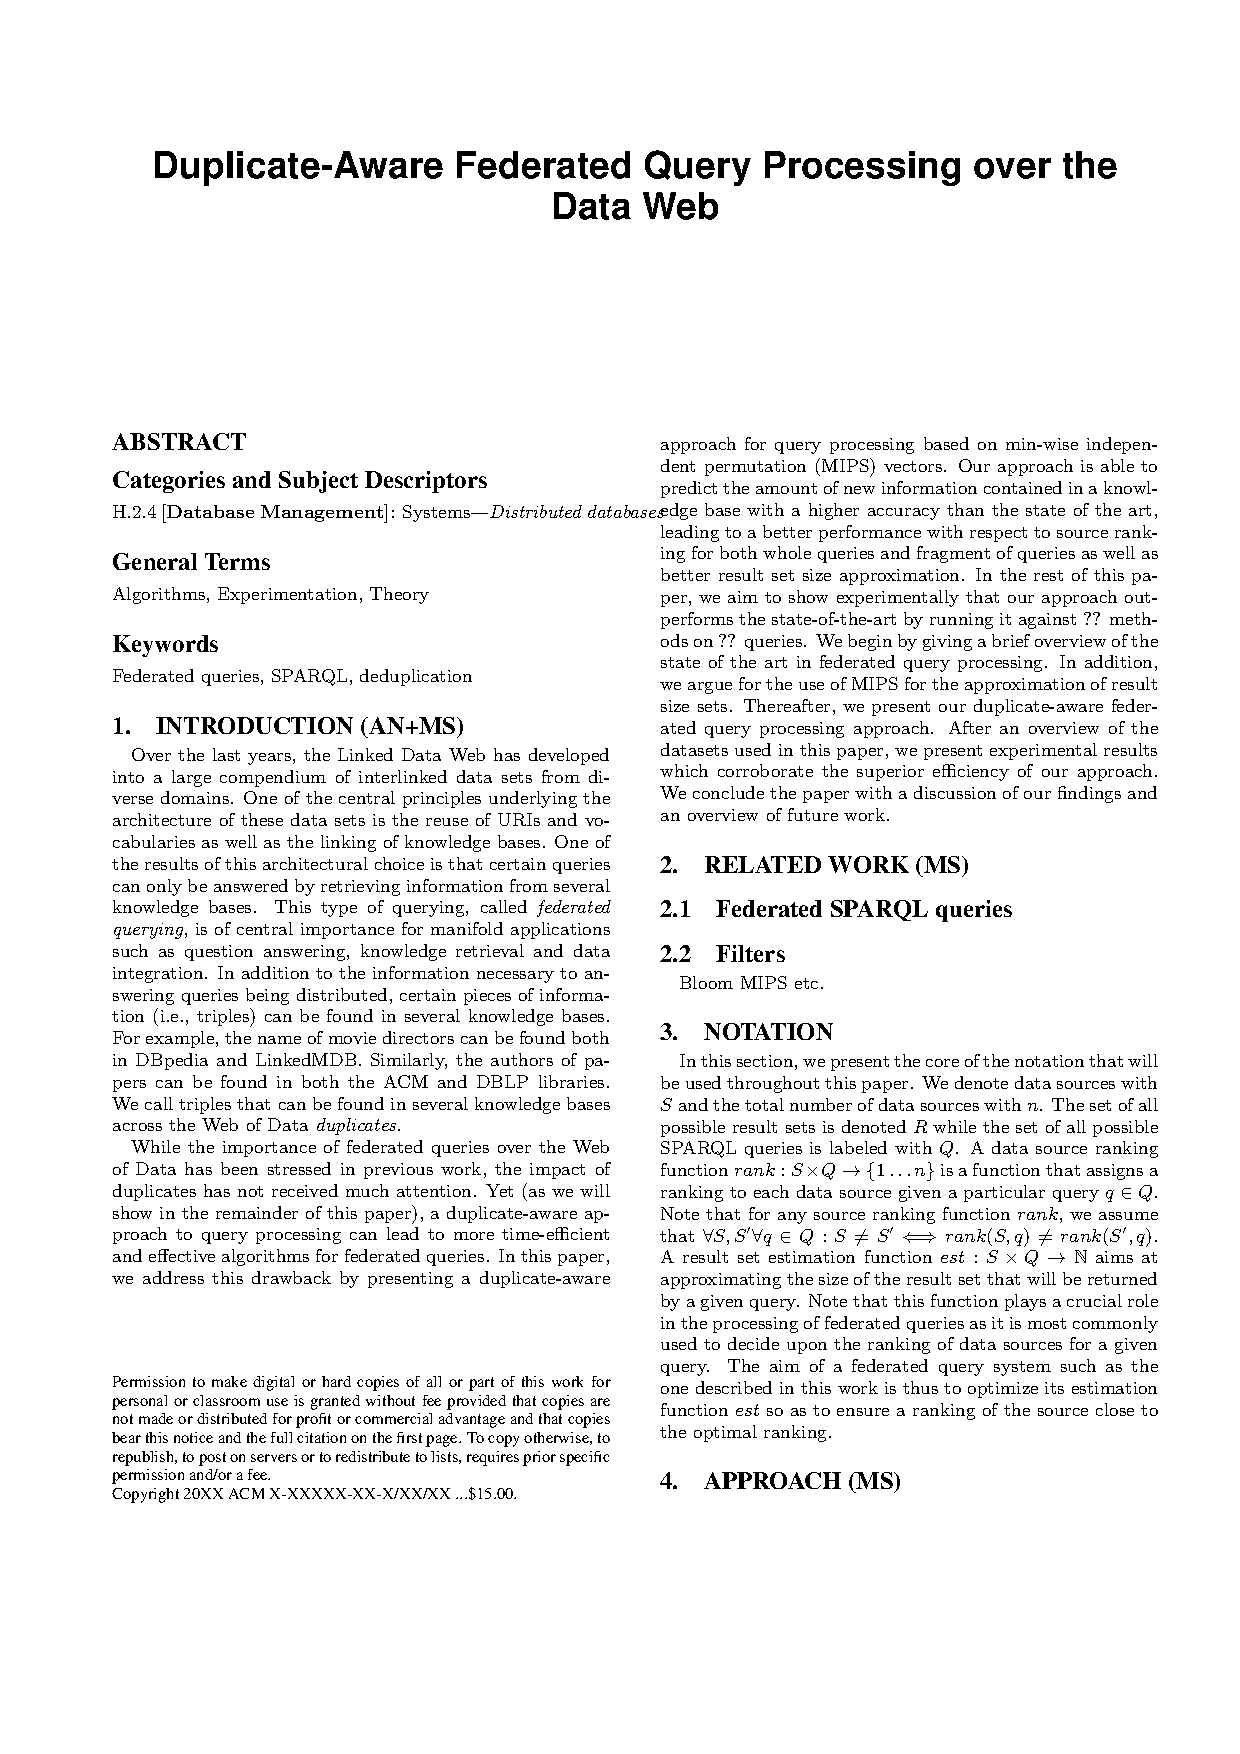
\includegraphics[scale=0.53]{img/mips} 
\par\end{centering}
%\centering Resemblance($S_A,S_B) = \dfrac{|S_A \cap S_B|}{|S_A \cup S_B|}$\\
%\left(\frac{a^{2} + b^{2}}{c^{3}} \right) = 1

\caption{Min-Wise Independent Permutations}
\end{figure}

\subsection{Source Selection}
A SPARQL query contains one or more basic graph patterns. Similar to DARQ, our query planning
step is performed separately for each basic graph pattern.
The source selection algorithm used in DARQ for
a query simply matches all triple patterns against the capabilities
of the data sources. The matching compares the predicate in a triple
pattern with the predicate defined for a capability. 

Let \emph{S =$\{(s_1,C_1),..,(s_n,C_n)\}$ } be a set of all indexed data sources \emph{$s_1..s_n$} and their capabilities \emph{$C_1..C_n$,} where \emph{$C_i = \{(p_i, mipsv_i, sbjsel_i, objsel_i, totTrpl_i)\}$}.
Let \emph{BGP} be a set of triple
patterns in a filtered basic graph pattern. The result of the source
selection is a set of data sources $D_j$ for each triple
pattern $t_j = (s_j, p_j, o_j)$ $\in$\ \emph{BGP} such that 

\begin{center}
$D_j$ = \{s$|$(s,C) $\in$ \ S $\wedge$ \ $\exists$
\ $p_j$ $\in$ \ C \}
\par\end{center}

We extend the DARQ source selection algorithm by comparing MIPs vectors
 for duplicates. For a triple pattern, we compare the MIPs
vectors of all the relevant data sources for possible duplicates.
A specific source \emph{s} is only added to the set of capable sources $D_j$,
if it is able to produce a number of new results above a specific threshold value
pre-defined for final source selection. For a triple \emph{t $\in$\ BGP} and a dataset \emph{s $\in$\ S}, if the value of new results generated
is less than the threshold, \emph{s} is ignored from set $D_j$. For 100\%\ recall the threshold value should be 1. Which means if a source is able to produce a single triple, it will be added to the set of capable sources. For sufficient (not complete) record retrieval the threshold can be fixed to any number greater than 1. For all of the 79 queries in this work, our threshold value is 1. 

\subsection{Source Ranking} 
To show the importance of the duplicate-aware data source ranking (based on the amount of duplicate-free records retrieved), suppose we have a triple pattern query\emph{q} shown in Listing 2  and \emph{$ ds_1, ds_2, ds_3 $} are the data sources capable of answering that query. If we apply DARQ source selection algorithm we will get all 3 datasets as the list of capable sources. Let us assume that $ds_1$ has a total of 50 triples satisfying \emph{q}, $ds_2$ and $ds_3$ each have 40 triples satisfying the query. Further suppose that 25 of the $ds_3$ triples are duplicated at $ds_1$ while remaining 15 are duplicated at $ds_2$. The DARQ sub-query generator would forward the query to all 3 data sources. Thus, it would generate unnecessary network traffic to retrieve the data contained in $ds_3$. 
The integration time would also be suboptimal as the $ds_3$ records would have to be joined to the results of the two other data sets during the final result set compilation. Now if we apply duplicate-aware source ranking approach, which would select $ds_1$ as first, $ds_2$ as second and would skip $ds_3$, we would only send two sub-queries (one to $ds_1$and one to $ds_2$) and thus improve both network traffic and integration time.

Similar to DARQ, our system make use of the triple-by-triple sub-query federation, therefore it is important to have a duplicate-aware triple pattern source ranking algorithm for sub-query escaping. We present this triple pattern source ranking algorithm in the next section. 

\begin{lstlisting}[caption = {A single triple pattern query},basicstyle={\tiny},frame = {single},stringstyle={\ttfamily}]
 SELECT ?o
   WHERE
    {
        ?s  <p1> ?o .
    }
\end{lstlisting}

\subsubsection{Triple Pattern Source Ranking}
Algorithm 1 shows the single triple pattern source ranking. For a triple \emph{t(s,p,o) $\in$ T } the set of capable data sources \emph{D} is obtained using the source selection algorithm explained in previous section. The source \emph{d $\in$ D} which has the highest \emph{totTrpl} value in the matched capability \emph{C(p, mipsv, sbjsel, objsel, totTrpl)} is selected as first in the rank. The union and intersection of \emph{MIPs Vectors} is explained in section 4.3. In order to get the accurate result set estimate, we multiply \emph{sbjsel, objsel $\in C$} to the \emph{orignal size} of the \emph{MIPs Vectors} if \emph{subject} or \emph{object} of the triple pattern is bound respectively. The same is true for rank 1 dataset selection. However, the multiplication is performed with \emph{totTrpl} of mached capability instead of \emph{orignal size}. 

It is important to note that the number of elements in the MIPs vector may be different from its \emph{orignal size}. The \emph{orignal size} is the number of elements in the \emph{ID set} over which we applied \emph{N} random permutations to get the MIPs Vector as explained in MIPs section. In the line 24 we set the threshold value to 1 in order to get 100\% recall. For each triple pattern $t_j = (s_j, p_j, o_j)$ in the query \emph{q} $\in$ \emph{Q}, we apply the Algorithm 1 to get a set of selected capable data sources \emph{$D_{s_j}$} which is used in sub-query generating algorithm explained in Section 4.6.

\begin{algorithm}[float,tiny]
\caption{triple pattern source ranking}
\begin{algorithmic} [1]
\REQUIRE  t(s,p,o) $\in$ T  //triple pattern 
\STATE D = getCapableSources(t) //all sources capable of answering triple \emph{t}
\STATE $rank_1Source$ = getMaxSizeSource(D,t)
\STATE rnkNo = 1
\STATE unionMipv = $rank_1Source$.getMIPv(t) 
\STATE $D_{s}$[rnkNo] = selectedSource
\STATE D = D - \{selectedSource\}
\STATE rnkNo = rnkNo+1
\WHILE{$D \neq \emptyset$}
\STATE selectedSource = null
\STATE maxDistinctRecords =0
\FOR {each $d_i$ $\in$ D }
\STATE mipv = $d_i$.getMipv(t)
\IF  {\emph{s} is bound in \emph{t}} 
\STATE mipv.orignalSize =mipv.orignalSize*$d_i$.getSbjSel(t)
\ELSIF {{\emph{o} is bound in \emph{t}} }
\STATE mipv.orignalSize =mipv.orignalSize*$d_i$.getObjSel(t)
\ENDIF

\STATE overlap = unionMipv.intersectionSize(mipv)
\STATE distinctRecords = mipv.getOrignalSize()-overlap
\IF{distinctRecords > maxDistinctRecords}
\STATE selectedSource = $d_i$
\STATE maxDistinctRecords = distinctRecords
\ENDIF
\ENDFOR
\IF{maxDistinctRecords $\geqslant$ 1}
\STATE $D_{s}$[rnkNo] = selectedSource
\STATE selectedMipv = selectedSource.getMipv(t)
\STATE  unionMipv =  unionMipv.union(selectedMipv)
\STATE rnkNo = rnkNo+1
\ENDIF
\STATE D = D - \{selectedSource\}
\ENDWHILE
\RETURN $D_{s}$  //rank wise selected sources
\end{algorithmic}
\end{algorithm}
%<<<<<<< HEAD
%\subsubsection{Join Source Ranking (this section is not well written)}
%Similar to DARQ, we perform individual triple based sub-query federation. Consequently, triple pattern source ranking is most important for sub-query escaping. The advantage of this approach is that if a data source is not capable of answering the complete query, it may produce enough results for a specific sub-set of query triples. For the comparison purpose we propose a complete query source ranking which works as follow: For a star shaped queries, the overall result set is bound by the triple with lowest number of estimated records. Therefore, we perform the source ranking for that triple (using Algorithm 1) and use this as complete query ranking. The lowest records query triple can be estimated using the rank 1 source selection explained in previous section. However, this time we are looking for a source which has the lowest estimated value of all. For path shaped queries the total records are bound by the triple which has \emph{subject} variable equal to the \emph{object} of the previous query triple. For example the result set in the query given in Listing 2, is bound by the second triple in which the \emph{object} variable in the first triple is used as \emph{subject} in the second triple. Therefore, we perform the triple pattern ranking for second triple and use this as ranking for complete query.
%%\lstinputlisting[caption=.,label=ex:q1, language=SPARQL]
%\begin{lstlisting}[caption = {A P-1 query example},frame = single,language=SPARQL]
 %SELECT ?s 
%=======
\subsubsection{Join Source Ranking}
 As mentioned earlier, we perform individual triple based sub-query federation. Consequently, triple pattern source ranking is most important for sub-query escaping. The advantage of this approach is that if a data source is not capable of answering the complete query, it may produce enough results for a specific sub-set of query triples. For the comparison purpose we propose a complete query source ranking which works as follow: For a star shape queries like the query given in Listing 4, the overall result set is bound by the triple with lowest number of estimated records. Therefore, we perform the source ranking for that triple (using Algorithm 1) and use this as complete query ranking. The lowest records query triple can be estimated using the rank 1 source selection explained in previous section. However, this time we are looking for a source which has the lowest estimated value of all. For path shaped queries the total records are bound by the triple which has \emph{subject} variable equal to the \emph{object} of the previous query triple. For example the result set in the query given in Listing 3, is bound by the second triple in which the \emph{object} variable in the first triple is used as \emph{subject} in the second triple. Therefore, we perform the triple pattern ranking for second triple and use this as ranking for complete query.
\begin{lstlisting}[caption = {A P-1 query example},basicstyle={\tiny},frame = {single},language=SPARQL,stringstyle={\ttfamily}]
 SELECT ?o1 
   WHERE
    {
        ?s  <p1> ?o .
        ?o  <p2> ?o1
    }
\end{lstlisting}

\subsection{Sub-query generation}
 The sub-query generation algorithm is similar to the one presented in DARQ. However, instead of using all capable sources, we use selected data sources (obtained from Algorithm 1) for the sub-query generation. Let \emph{(T,s)} be a sub-query, where \emph{T} is a set of triple patterns, and \emph{s} is the data source that can answer this sub-query. The sub-query generation is shown in Algorithm 2. If a triple pattern \emph{$t_j$} matches exactly one data source \emph{($D_{s_j}$ = \{s\})} then the triple will be added to the set of sub-queries for this data source. All triples in this set will be sent to the data source in one sub-query. If a triple matches more than one data sources then the triple will be sent individually to all matching data sources
in separate sub-queries. After the sub-queries are generated, the federator sends all of them to the optimizer for further optimization, before the federation. Our optimizer and data integrator module is similar to DARQ. 
\begin{algorithm}[float,tiny]
\caption{sub-query generation}
\begin{algorithmic} [1]
\REQUIRE T = \{ $t_1,..,t_n$\} \\
 S = \{$D_{s_1}$,..,$D_{s_n}$\} // sets of data sources obtained from algorithm 1  
\STATE \emph{sub-queries} = $\emptyset$, \emph{seperateSub-queries} = $\emptyset$
\FOR  {each $t_i$ $\in$ T} 
\IF {$D_{s_j}$ = \{s\}}
\STATE q = \emph{queries.getQuery(s)}
\IF   {q not null }
\STATE q.T = q.T + $t_i$
\ELSE 
\STATE \emph{sub-queries} = \emph{sub-queries} + (\{$t_i$\},s)
\ENDIF
\ELSE 
\FOR {each $s_j$ $\in$ $D_{s_j}$}
\STATE \emph{seperateSub-queries} = \emph{seperateSub-queries} + (\{$t_i$\},s)
\ENDFOR
\ENDIF
\ENDFOR
\RETURN \emph{sub-queries} $\cup$ \emph{seperateSub-queries} //Return all sub-queries
\end{algorithmic}
\end{algorithm}
\section{Experiments and Results}
The goal of our experiments was to assess how well our duplicate-aware solution performs in terms of result set recall, ranking of data sources and runtime.
We compared our approach with DARQ, a well-known, publicly available and widely used federated query execution engine.\footnote{We refrained from comparing with the approach presented in~\cite{key-5} because it connot deal with the partly fragmented data which is generated in our experiments.}
We also compared our approach with a simulation of the optimal duplicate-unaware (DU) approach, where (1) the result set estimation of carried is carried out regardless of the overlap between data source and each source containing at one relevant triple is queried.
In the following, we describe our experimental setup in detail and contrast the results achieved by each of the approaches.
All data used in this evaluation is either publicly available or can be found at the project webpage.\footnote{\url{https://sites.google.com/site/dupawarefedqueries/}}
\subsection{Experimental Setup}

\subsubsection{Datasets}
Within our experiments, we used the four datasets described in Table \ref{tab:datasets}.
The first data set, Diseasome,
%\footnote{\url{http://www4.wiwiss.fu-berlin.de/diseasome/diseasome_dump.nt.bz2}} 
contains diseases and disease genes linked by disease-gene associations.
The Publication data set is the Semantic Web Dog Food data set\footnote{\url{http://data.semanticweb.org/}} and contains information on publications, venues and authors of publications.
The Geo data set resulted from retrieving the portion of triples from DBpedia that maps resources to their geo-coordinates\footnote{\url{http://wiki.dbpedia.org/Downloads38\#geographic-coordinates}.}.
Finally, LinkedMDB~\footnote{\url{http://queens.db.toronto.edu/~oktie/linkedmdb}} is the RDF version of IMDB and contains amongst others a large number of actors, movies and directors.
We chose data sets of different data sizes to assess the scalability of our approach.
The size of the MIPS vectors was set to achieve a compression ratio between 96\% and 98\%, which is similar to that used in previous work~\cite{key-5}.

Given that we wanted to emulate fragmented data sets distributed across several sources, we distributed each of the data sets $D$ across $n=10$ data sources (which we also call ``slices'').
The first step of this process consisted of deciding on the size of the slices.
We controlled the maximal size difference between the different slices by setting the \emph{discrepancy factor} $d$, which is given by
\begin{equation}
d = \max\limits_{1 \leq i \leq n} |S_i| - \min\limits_{1 \leq j \leq n} |S_j|,
\end{equation}
where $S_i$ stands for the i$^{th}$ slice. 
Given a value of $d$, we computed the sizes of the slices by assigning them random sizes such that $\sum\limits_{i} |S_i| = D$ and $\forall i \forall j\,i \neq j \rightarrow ||S_i| - |S_j|| \leq d$.
The data was then distributed across the 10 data sources by partitioning the input according to the pre-computed sizes of the slices.
Finally, we picked $m$ out of the $n$ data sources randomly ($m < n$) and redistributed their content across all $n-m$ remaining data sources .
We set $d$ to values between ca 1.6\% and 2.8\% of the triples.
Note that the value of $d$ was increased with increasingly larger data sets.

\begin{table*}
\centering
\begin{tabular}{lrrrrrrrrr}
\hline
Dataset & Size  & Summary 	& CR   & Slices & Discrepancy & Duplicate  & Duplicate & Total 	& Sum. Gen. \\
				& (MB) 	& Size (MB) & (\%) &	  		 &  					 & Slices 		& Datasets 	& Triples & Time (sec)\\
\hline
Diseasome 			& 18.6 	& 0.64 	& 96 & 10 & 1,500 		& 1 & 10 			& 91,122 & 9\\
Publication 						& 39.0	& 1.15 	& 97 & 10 & 2,500 		& 1 & 10 			& 234,405 & 16\\
Geo 						& 274.1 & 4.66 	& 98 & 10 & 50,000 	& 2 & 5,8				& 1,900,006 & 1302\\
LinkedMDB 			& 448.9 & 7.9 	& 97 & 10 & 100,000 	& 1 & 2 			& 3,579,616 & 1837\\
\hline
\end{tabular}
\caption{Overview of datasets. Size gives the magnitude of the data sets in MB. Summary size is the size of the correspoding MIPS. Slices is the number of data sources used during the experiments. Discrepancy gives the absolute value of the discrepancy used for the given experiment. CR stands for Compression Ratio.}
\label{tab:datasets}
\end{table*}


\subsubsection{Queries}
We used three main types of queries in our experiments: basic graph patterns (BGP), star-shaped and path-shaped queries.
\emph{Basic graph pattern} (BGP) queries consist of exactly one triple pattern in the query.
Star-shaped and path-shaped queries are defined as in~\cite{key-5}: \emph{star-shaped queries} (denoted by S-k) have one variable as subject and contained k joins, i.e., (k+1) triple patterns.
An example of a S-1 star-shaped query is given in the listing below.
\begin{lstlisting}[caption = {A S-1 query example},basicstyle={\tiny},frame = single,language=SPARQL]
 SELECT ?s 
   WHERE
    {
        ?s  <p1> ?o1 .
        ?s  <p2> ?o2
    }
\end{lstlisting}
Path-shaped queries (denoted by P-k) were generated by using a random walk approach to generate a path of length $k$ (see Listing 2 for an example of a P-1 query). 
Note that previous work has shown that these query shapes are the most common shapes found in real-world RDF queries~\cite{key-35}.
Overall, our benchmark data consisted of 79 queries as shown in Table~\ref{tab:queries}.
Some query shapes could not be used on certain datasets due to the topology of the ontology underlying the datasets not being permissive for such queries. 
For example, P-1 queries could not be sent to the Geo datasets because it only contained object properties.

\begin{table}
\centering
\begin{tabular}{lrrrrrrr}
\hline
Dataset 		& BGP  & S-1 & S-2 & P-1 & P-2 & P-3 & Total \\\hline
Diseasome 			& 5 & 5 & 5 & 4 & 5 & 2 & 26 \\
Geo  & 5 & 5 & 5 & 0 & 0 & 0 & 15 \\
LinkedMDB 			& 5 & 0 & 0 & 0 & 0 & 0 & 5 \\
Publication 		& 5 & 5 & 5 & 7 & 7 & 4 & 33 \\\hline
Total 					& 20 & 15 & 15 & 11 & 12 & 6 & 79\\
\hline
\end{tabular}
\caption{Distribution of query types across datasets}
\label{tab:queries}
\end{table}

\subsubsection{Metrics}
We used two metrics to compare our approach with the state of the art.
First, we measured the mean squared error of each approach tested with respect to their result set evaluation as follows:
For each query $q_i$, each source $S_i$ contained a number $R_i(q_i)$ of non-duplicate results.
Each of the approaches generated an approximation $\tilde{R}_i(q_i)$ of $R_i(q_i)$.
The mean squared error with respect to the result set size (short $RSMSE$) was then computed as follows:
\begin{equation}
RSMSE = \frac{1}{|Q|}\sum\limits_{q_i \in Q}|R_i(q_i) - \tilde{R}_i(q_i)|^2.
\end{equation}
In addition to the RSMSE, we also computed how well the approaches were able to rank the data sources with respect to the unseen triples they would return for a given query.
Given the ideal ranking $rank(S_i, q_j)$ of each data source $S_i$ for each query $q_j$ and the ranking $\tilde{r}(S_i, q_j)$ achieved by a given approach, we computed the mean squared ranking error (short $RankMSE$) as follows:
\begin{equation}
RankMSE (q_j) = \frac{1}{|\mathfrak{S}|}\sum\limits_{S_i}|rank(S_i, q_j) - \tilde{r}(S_i, q_j)|^2.
\end{equation}
\begin{equation}
RankMSE  = \frac{1}{|Q|}\sum\limits_{q_j  \in Q}RankMSE(q_j).
\end{equation}
For both measures, the higher values the worse the performance of the federated query approach.

\subsection{Results}

\subsubsection{Result Set Estimation and Ranking}
The RSMSE results are shown in Figures~\ref{fig:rsmse} while the ranking results are shown in Figure~\ref{fig:rank}.
In each figure, we compared the results of the approaches w.r.t. both the whole input query and to each of the triples patterns contained in the input queries.
Our results clearly show that we outperform the state of the art w.r.t. both result set estimation and ranking.
In particular, our estimation of the result set sizes is approximately 4 orders of magnitude better than DARQ's and DU's. 
This is due to our approach being able to capture the existence of duplicates in the data sets and thus to better approximate the number of new results that can be expected from  an endpoint.
As expected, the ranking error for datasets decreases when carrying the ranking of data sources at triple pattern level instead of query level (see Figures~\ref{fig:rsmse}).
This is simply due to the overall error increasing when combining the several triple patterns to a query.
The same overall behavior is also displayed when considering the result set estimation error (see Figures~\ref{fig:rank}). 
%Interestingly, the approximation of our approach is slightly poorer on star-shaped queries (approx. 0.2 on S-2 queries).
%This is a result of our approach to generating the estimations for whole query, which is carried out by using the lower bound of the estimation of single query patterns in the query. 
%Small errors in the estimation of the size of the result size can thus lead to minor absolute errors.



As stated before, we used a compression ratios between 96\% and 98\% across all experiments. 
The main advantage of such a high compression ratio is the small size of the index generated by our approach. 
Yet, higher compression ratios also lead to cruder approximations and thus to larger error margins of the number of duplicate-free triples in each data source.
Consequently, the $RSMSE$ and $RankMSE$ of our approach can be high for queries whose sub-queries lead to result sets of similar magnitude.
We wanted to know whether a decrease of the reduction ratio leads to our approach being able to capture even small differences across the sizes of the sub-query result sets.
We thus studied the effect of decreasing the compression ratio on the $RSMSE$ and $RankMSE$ for such a query (which one)?.
Our results in Table~\ref{tab:compression} suggest that MIPS vectors can successfully detect even small differences in the sizes of the result sets when given a sufficiently small compression ratio.


\subsubsection{Recall and Runtime}

Table~\ref{tab:recall} shows the recall achieved by MIPS and DARQ in relation to the number of slices taken into consideration. 
Our results display the superiority of our ranking function, which is always able to achieve full recall of 1 by querying 9 from the 10 available data sources. 
In contrast, DARQ always has to visit all data sources to achieve a comparable recall. 
%One of the main advantages of systems that process federated queries at sub-query-level is that refrain for sending sub-queries to all available data sources if these sources appear not to contain relevant information. 
%The advantage of this strategy obviously lies in superior runtimes and better resource management (less network traffic, smaller space requirements, etc.).
We measured the number of sub-query executions that could be escaped by our approach without any loss in recall. 
The results shown in Table~\ref{tab:escaped} clearly demonstrate that our approach can effectively reduce the total number of queries executed overall.
Especially, on BGP queries, we were able to escape up to 10 sub-queries. 
Our approach was most successful on star-shaped queries, where up to 21 sub-queries could be escaped. 
The better ranking function also leads to a superior overall runtime as shown in Figure~\ref{fig:runtime_recall}.
In average, our approach requires solely between 79.85\% (S-2 queries) and 93.46\% (P-1 queries) of the runtime of DARQ to retrieve the complete result set to each query.

\begin{figure*}
\centering
\begin{subfigure}[b]{0.45\textwidth}
                \centering
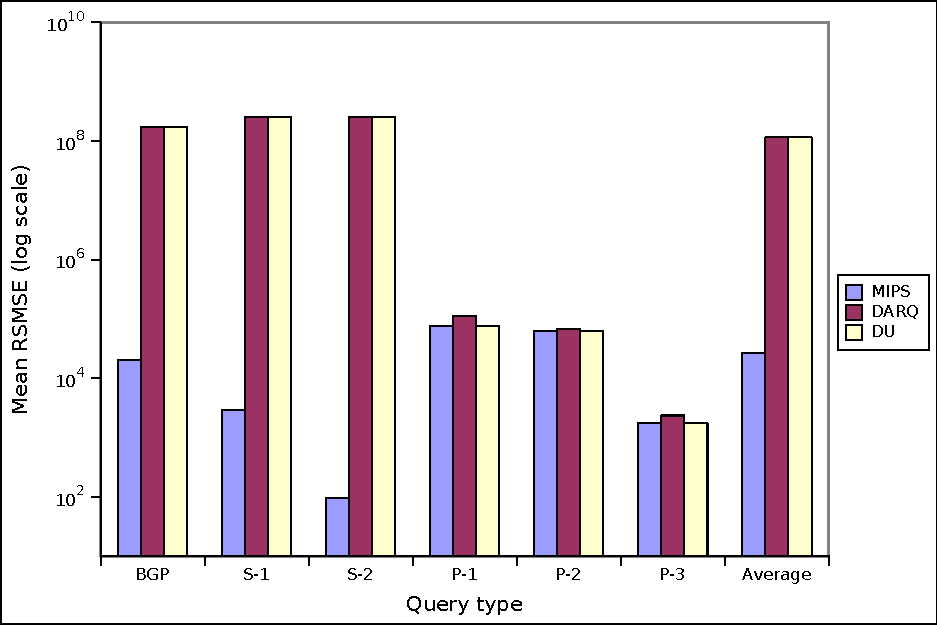
\includegraphics[width=\textwidth]{img/querywise_rse}
                \caption{RSMSE for query-wise selection}
                \label{fig:rsmseQuery}
        \end{subfigure}
\begin{subfigure}[b]{0.45\textwidth}
                \centering
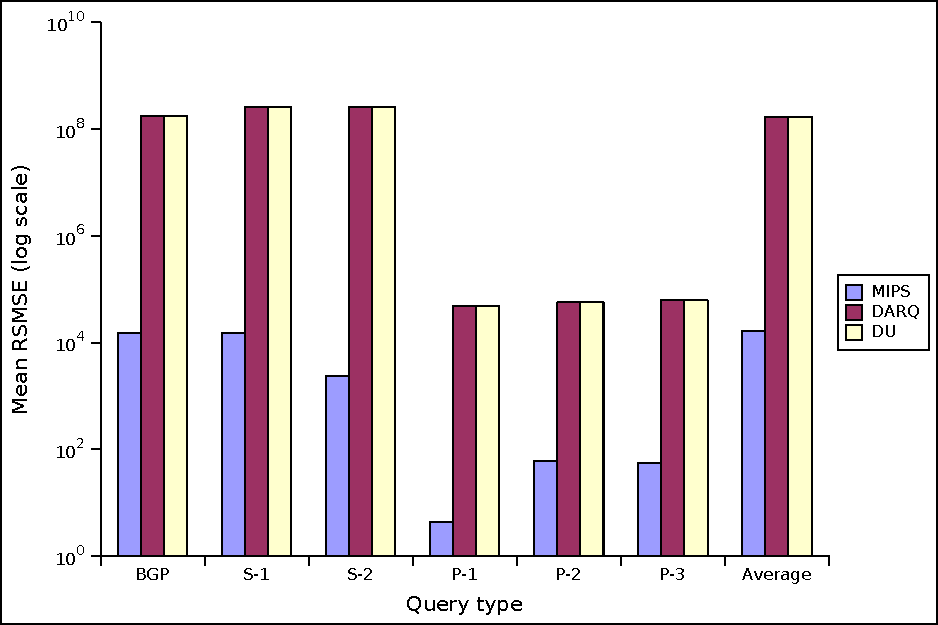
\includegraphics[width=\textwidth]{img/subquerywise_rse}
                \caption{RSMSE for subquery-wise selection}
                \label{fig:rsmseSubquery}
        \end{subfigure}
\caption{Mean squared errors with respect to result set evaluation across six query types}
\label{fig:rsmse}
\end{figure*}

\begin{figure*}
\centering				
\begin{subfigure}[b]{0.45\textwidth}
                \centering
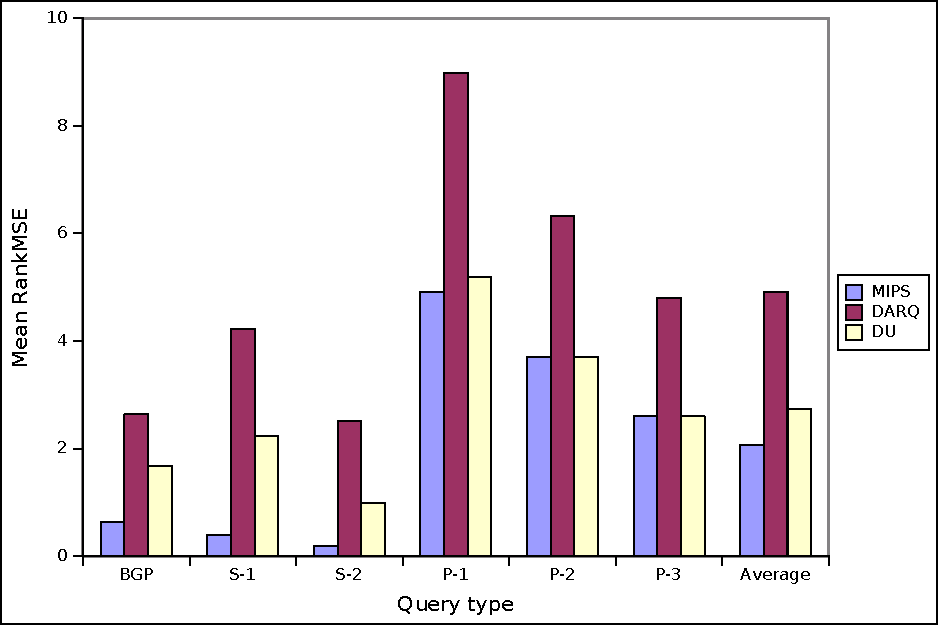
\includegraphics[width=\textwidth]{img/querywise_ranking}
                \caption{RankMSE for query-wise selection}
                \label{fig:rankQuery}
        \end{subfigure}			
				\begin{subfigure}[b]{0.45\textwidth}
                \centering
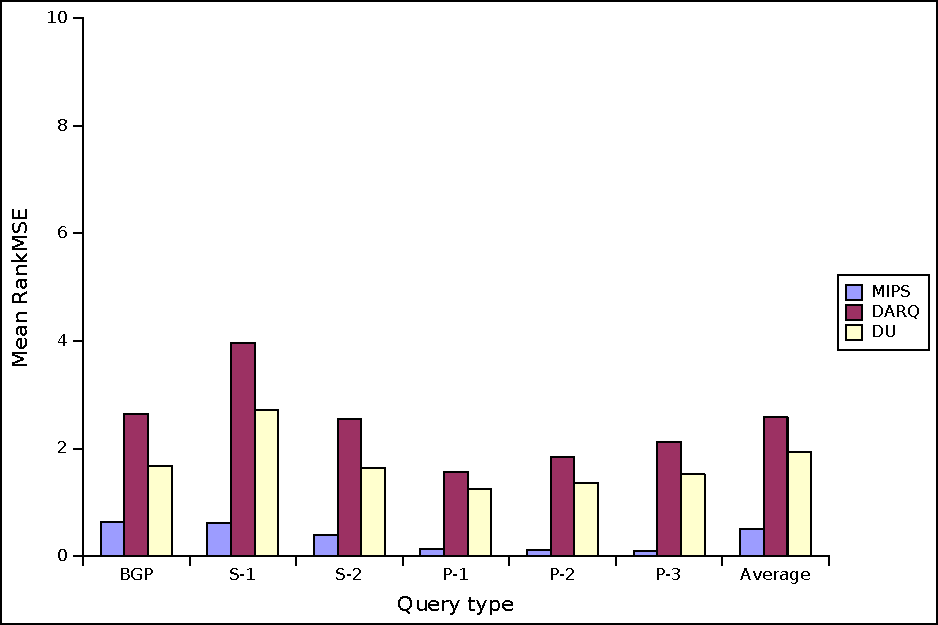
\includegraphics[width=\textwidth]{img/subquerywise_ranking}
                \caption{RankMSE for subquery-wise selection}
                \label{fig:rankSubquery}
        \end{subfigure}
\caption{Mean squared errors with respect to ranking across six query types}
\label{fig:rank}
\end{figure*}


\begin{table}
\centering
\begin{tabular}{rrr}
\hline
Compression Ratio		& $RSMSE$	& $RankMSE$ \\\hline
97\%	& $253.9 \times 10^6$	& 3.4 \\
94\%	& $33.3 \times 10^6$	& 0.6 \\
91\%	& 0					&	0 \\\hline
\end{tabular}
\caption{Effect of compression ratio}
\label{tab:compression}
\end{table}


\begin{table}
\centering
\begin{tabular}{lrrrrrrr}
\hline
Dataset		&BGP 	&S-1&S-2&P-1&P-2&P-3&Total \\\hline
Diseasome				&7		&21	&21	&8	&20	&12	&89\\
Geo 	&10		&15	&23	&0	&0	&0	&48\\
LinkedMDB				&5		&0	&0	&0	&0	&0	&5\\
Publication			&1		&2	&5	&0	&0	&0	&8\\\hline
Total 					&23		&38	&49	&8	&20	&12	&150 \\\hline
\end{tabular}
\caption{Distribution of sub-query escaped by our approach}
\label{tab:escaped}
\end{table}


%\subsubsection{Execution Time}
%\subsubsection{Size of MIPS vectors (on largest dataset)}
\section{Conclusion and Future Work}
In this paper, we presented an approach for duplicate-aware federated SPARQL querying.
Our approach combines object and subject selectivity with MIPs to estimate the number of duplicate-free result subsets.
Based on this estimation, it can select relevant data sources for a given query, rank these data sources according to the magnitude of relevant triples they contain and finally query them so as to maximize its recall.
We compared our approach with DARQ and a simulation of an perfect duplicate-unaware SPARQL federated query engine and showed that we achieve lower mean squared errors with respect to both the estimation of the result set sizes and the ranking of data sources.
Our results suggest that our approach can be easily adapted to scenarios where accurate approximations of result set sizes are required.
Moreover, the execution time of our approach was shown to be superior to that of the state of art's.
Our approach is also able to generate less network traffic by escaping sub-queries that would not lead to non-duplicate result sets.
In future work, we will extend our approach by combining it with tiem-efficient duplicate detection systems such as LIMES~\cite{key-26}. 
By these means, we will enable our engine to merge facts which are expressed in different vocabularies or by using different URIs for the same real-world entity.

\begin{table*}
\centering
\begin{tabular}{rrrrrrrrrrrrr}
\hline
Rank		 & \multicolumn{2}{c}{BGP}	& \multicolumn{2}{c}{S1}	&\multicolumn{2}{c}{S2}	&\multicolumn{2}{c}{P1}	& \multicolumn{2}{c}{P2}	& \multicolumn{2}{c}{P3} \\
	& MIPS & DARQ & MIPS & DARQ & MIPS & DARQ & MIPS & DARQ & MIPS & DARQ & MIPS & DARQ \\\hline
1 & 29,22 & 19,22 & 26,53 & 24,42 & 30,69 & 30,69 & 18,12 & 15,67 & 24,60 & 21,99 & 31,60 & 29,30 \\
2 & 49,61 & 39,50 & 46,20 & 39,67 & 52,15 & 49,70 & 34,04 & 31,49 & 38,84 & 38,56 & 43,78 & 45,02 \\
3 & 67,48 & 61,78 & 60,90 & 54,78 & 66,48 & 59,96 & 50,28 & 49,23 & 55,74 & 53,16 & 61,86 & 56,76 \\
4 & 78,44 & 72,68 & 70,75 & 63,86 & 76,60 & 71,49 & 65,71 & 64,04 & 72,25 & 69,11 & 80,17 & 73,72\\
5 & 85,65 & 79,26 & 79,76 & 74,32 & 83,64 & 80,54 & 77,24 & 79,87 & 83,04 & 86,11 & 90,45 & 91,74\\
6 & 90,54 & 84,00 & 86,67 & 79,59 & 89,90 & 86,76 & 82,28 & 83,75 & 87,69 & 89,95 & 94,48 & 95,70\\
7 & 94,68 & 87,25 & 92,94 & 85,61 & 94,88 & 90,22 & 85,56 & 87,17 & 89,99 & 92,08 & 95,59 & 96,73\\
8 & 99,40 & 89,38 & 98,62 & 89,98 & 99,35 & 93,43 & 87,71 & 89,29 & 91,47 & 93,31 & 95,70 & 97,53\\
9 & 100,00& 97,95 & 100,00& 96,52 & 100,00& 97,06 & 100,00& 94,97 & 100,00& 97,15 & 100,00& 99,26\\
10& 100,00& 100,00& 100,00& 100,00& 100,00& 100,00& 100,00& 100,00& 100,00& 100,00& 100,00& 100,00\\\hline
\end{tabular}
\caption{Comparison of recall on top-k data sources (in \%).}
\label{tab:recall}
\end{table*}

\begin{figure*}
\begin{centering}
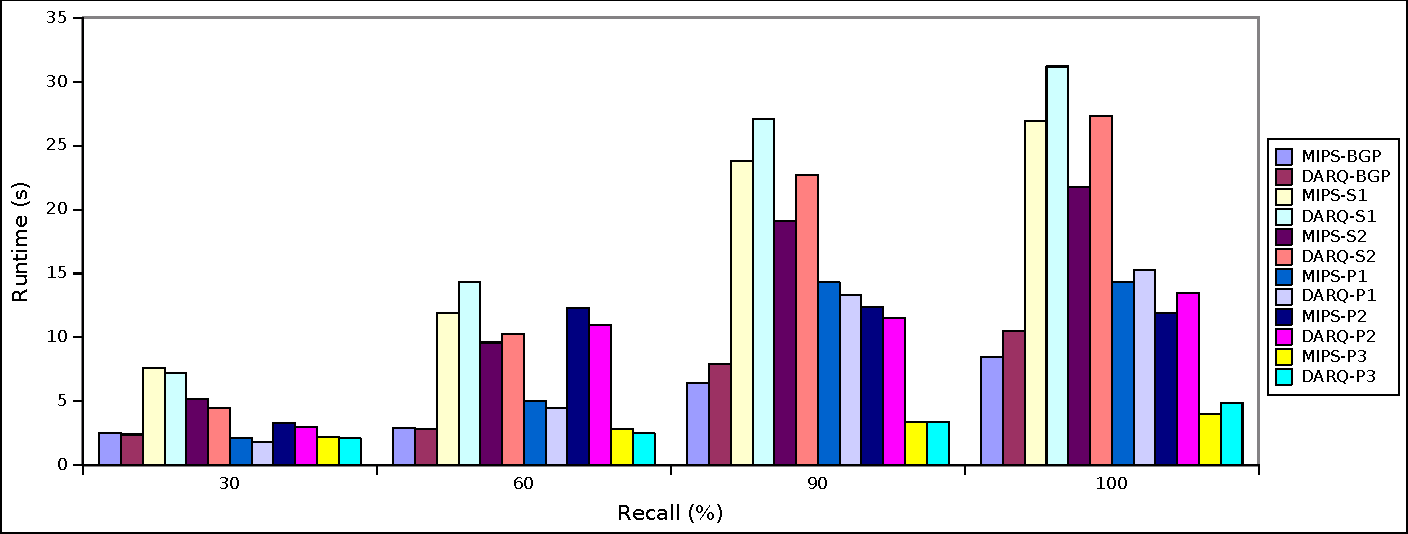
\includegraphics[width = 0.9\textwidth]{img/runtime_recall} 
\par\end{centering}
\caption{Comparison of runtimes for different recall values. The x-axis shows the recall (\%) achieved by our approach and DARQ on each of the six query types in our benchmark. }
\label{fig:runtime_recall}
\end{figure*}

\bibliographystyle{plain}
\bibliography{qa}

%\begin{thebibliography}{10}
%\bibitem{key-1}Stuckenschmidt, H., Vdovjak, R., Houben, G.J., Broekstra,
%J.: Index structures and algorithms for querying distributed rdf repositories.
%In: WWW'04. (2004).
%
%\bibitem{key-2}Quilitz, B., Leser, U.: Querying distributed RDF data
%sources with SPARQL. In: European semantic web conference on the semantic
%web: research and applications (ESWC 2008). LNCS, vol. 5021, pp. 524-
%538. Springer, Heidelberg (2008).
%
%\bibitem{key-3}Langegger, A., Waoay, W., Blaochl, M.: A semantic web
%middleware for virtual data integration on the Web. In: European semantic
%web conference on the semantic web: research and applications (ESWC
%2008). LNCS, vol. 5021, pp. 493-507. Springer, Heidelberg (2008).
%
%\bibitem{key-4}Hartig, C. O, Bizer, J.-C. Freytag. Executing SPARQL
%queries over the web of linked data. 8th International Semantic Web
%Conference (ISWC 2009).
%
%\bibitem{key-5}Harth, A., Hose, K., Karnstedt, M., Polleres, A.,
%Sattler, K.U. Umbrich, J.: Data summaries for on- demand queries over
%linked data. In: (WWW 2010), USA.
%
%\bibitem{key-6}Umbrich, J., Hose, K., Karnstedt, M., Harth, A., Polleres.:
%Comparing data summaries for processing live queries over Linked Data.
%In:(WWWJ 2011), special issue querying the data web. 
%
%\bibitem{key-7}Schwarte, .A, Haase, .P, Hose, .K, Schenkel, R, Schmidt,
%M.: FedX: Optimization Techniques for Federated Query Processing on
%Linked Data. In: 10th International semantic web conference (ISWC
%2011).
%
%\bibitem{key-8}Perez, J., Arenas, M., Gutierrez, C.: Semantics and
%Complexity of SPARQL. In: 4th International SemanticWeb Conference
%(ISWC), Athens, GA, USA (November 2006).
%
%\bibitem{key-9}Broder, A. Z., Charikar, M., Frieze, A. M., \& Mitzenmacher,
%M. (2000). Min-wise independent permutations. Journal of Computer
%and System Sciences, 60(3), 630-659.
%
%\bibitem{key-10}Bloom, B. H. (1970). Space/time trade-offs in hash
%coding with allowable errors. Communications of ACM, 13(7), 422-426.
%
%\bibitem{key-11}Mitzenmacher, M. (2002). Compressed bloom filters.
%In IEEE/ACM Transactions on Networking, 10(5), 604-612.
%
%\bibitem{key-12}Bender, M., Michel, S., Weikum, G., \& Zimmer, C.
%(2005). Minerva: Collaborative p2p search. In Proceedings of the (VLDB)
%conference (Demonstration).
%
%\bibitem{key-13}Parreira, J.X, Michel, S., Weikum, G.: p2pDating:
%Real life inspired semantic overlay networks for Web search. In: Journal
%of Information Processing and Management 43 (2007) 643-664.
%
%\bibitem{key-14} http://www4.wiwiss.fu-berlin.de/lodcloud/state/
%
%\bibitem{key-15}Y. Li and J. Hefl{}in. Using reformulation trees
%to optimize queries over distributed heterogeneous sources. In ISWC,
%pages 502-517, 2010.
%
%\bibitem{key-16}Z. Kaoudi, K. Kyzirakos, and M. Koubarakis. Sparql
%query optimization on top of dhts. In ISWC, pages 418-435, 2010.
%
%\bibitem{key-17}A. Deshpande, Z. G. Ives, and V. Raman. Adaptive
%query processing. Foundations and Trends in Databases, 1(1):1-140,
%2007.
%
%\bibitem{key-18} G. Ladwig and T. Tran. Linked data query processing
%strategies. In ISWC, pages 453-469, 2010.
%
%\bibitem{key-19}G. Ladwig and T. Tran. Sihjoin: Querying remote and
%local linked data. In ESWC (1), pages 139-153, 2011.
%
%\bibitem{key-20}Auer.S, Lehmann. J, Ngonga, A.C.: Introduction to
%Linked Data and Its Lifecycle on the Web. In: Reasoning Web. Semantic
%Technologies for the Web of Data, Pages 1-75, 2011.
%
%\bibitem{key-21}M. Acosta, M.-E. Vidal, T. Lampo, J. Castillo, and
%E. Ruckhaus. Anapsid: An adaptive query processing engine for sparql
%endpoints. In Proc. of International Semantic Web Conference (ISWC),
%2011.
%
%\bibitem{key-22}C. Buil-Aranda, M. Arenas, and O. Corcho. Semantics
%and optimization of the sparql 1.1 federation extension. In ESWC (2),
%pages 1-15, 2011.
%
%\bibitem{key-23}. M. Stoker, A. Seaborne, A. Bernstein, C. Keifer,
%and D. Reynolds. SPARQL Basic Graph Pattern Optimizatin Using Selectivity
%Estimation. In WWW, 2008.
%
%\bibitem{key-24}C. Basca and A. Bernstein. Avalanche: Putting the
%Spirit of the Web back into Semantic Web Querying. In The 6th International
%Workshop on SSWS at ISWC, 2010.
%
%\bibitem{key-25}O. Hartig. Zero-knowledge query planning for an iterator
%implementation of link traversal based query execution. In ESWC, pages
%154-169, 2011.
%
%\bibitem{key-26}Axel-Cyrille Ngonga Ngomo and Soren Auer. LIMES -
%A Time-Ecient Approach for Large-Scale Link Discovery on the Web of
%Data. In Proceedings of IJCAI, 2011.
%
%\bibitem{key-27} R. Isele, A. Jentzsch, and C. Bizer. Ecient Multidimensional
%Blocking for Link Discovery without losing Recall. In WebDB, 2011.
%
%\bibitem{key-28}Axel-Cyrille Ngonga Ngomo and Klaus Lyko. EAGLE:
%Ecient Active Learning of Link Specications using Genetic Programming.
%In: ESWC(2012).
%
%\bibitem{key-35}M. Morsey, J. Lehmann, S. Auer, and A.-C. {Ngonga Ngomo}.
%DBpedia SPARQL Benchmark - Performance Assessment with Real Queries
%on Real Data. In 10th Interna- tional Semantic Web Conference (ISWC2011),
%2011.
%
%\bibitem{key-36}Ntarmos, N. and Triantafillou, P. and Weikum, G.
%Distributed hash sketches: Scalable, efficient, and accurate cardinality estimation for distributed multisets. ACM Trans. Comput. Syst.
%January 2009,2:1--2:53.
%
%\bibitem{key-37}Polyzotis, Neoklis and Garofalakis, Minos. Statistical synopses for graph-structured XML databases. Proceedings of the 2002 ACM SIGMOD international conference on Management of data. 2002,358--369. 
%
%\bibitem{key-38}Natasha Drukh and Neoklis Polyzotis and Yossi Matias. Fractional XSKETCH synopses for XML databases. In Second International XML Database Symposium, XSym 2004, 189--203.
%
%\bibitem{key-39}Sebastian Michel, Matthias Bender, Peter Triantafillou,Gerhard Weikum. IQN Routing: Integrating Quality and Novelty in P2P Querying and Ranking. In Advances in Database Technology - EDBT 2006, 149-166.
%
%\bibitem{key-40}Moses S. Charikar.Similarity Estimation Techniques from Rounding
%Algorithms. Proceedings of the thiry-fourth annual ACM symposium on Theory of computing, 380--388.
%

%\end{thebibliography}

\end{document}

